%Chapter 3
\chapter{Research Design}
\label{Chapter3}
%-------------------------------------------------
\section{General Plan}
The overall goal of this experiment is to determine whether one meta learning
strategy within a given set can strictly dominate the others. The core elements
required in order to determine this are: (1) a set of meta learning strategies to be
compared, (2) sets of metabase datasets on which to apply the different strategies,
and (3) a means to evaluate the results so as to determine the relative performance
of the meta learners. The general flow of the program that constitutes this
experiment begins with a set of unprocessed datasets, then extracts the
meta features that are required to perform dataset clustering and to
run the active meta learning strategy. The program then constructs 10
meta learning bases with the elements in these sets chosen at random. A run with
every machine algorithm and dataset combination is then performed, with the
results being stored in the experiments database. Learning curves for each
dataset/algorithm combination are then crafted. Finally, enough information now
exists within the database to run the meta learning strategies
and extract results. This process is then repeated 30 times, with each run
constituting an individual sample. This produces enough information in order
to perform statistical analysis techniques to test the null hypothesis and
obtain a $p$ (the probability that the null hypothesis is true given our data)
value of 5 percent. A detailed explanation of the experiment steps follows now,
with a description of the statistical analysis to follow in Chapter 4.

\begin{figure}
  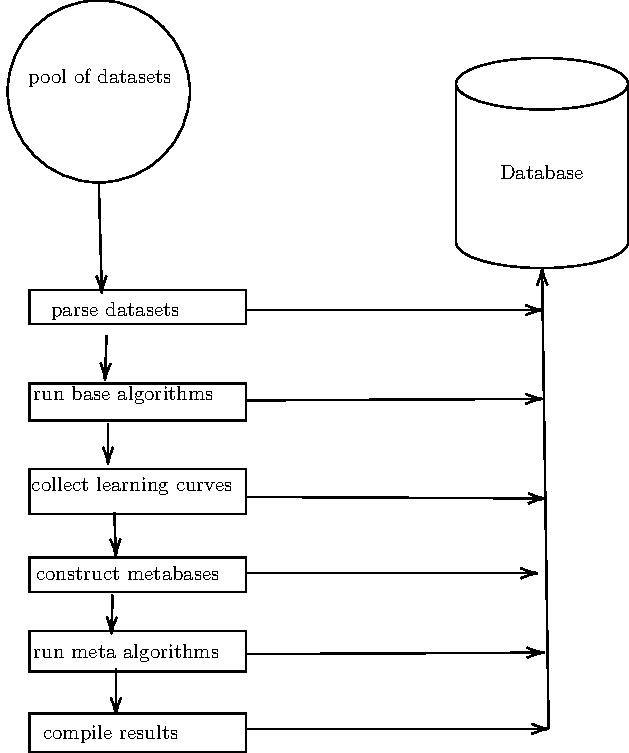
\includegraphics{Chapters/Images/MetaLearnerFLowchart/MetaLearnerFlowchart.pdf}
  \caption{A visual representation of this experiment's program flow}
\end{figure}

\section{Data Parsing}
The data used in this experiment come from the UCI Irvine Machine learning
repository, the obtainment of which was accomplished via the use of a bash
shell script that allowed the downloading of every dataset in the repository
all at once. To make use of a dataset from the repository, the algorithms used
in this experiment required a vector representation of the dataset currently
being analyzed; the data could not be used without first translating it into
this form. As such, I needed to do two things with the data before making use
of them: ensure that the data could be parsed into a vector via the use of a program,
then write a program in order to do this. The strategy I employed in order to
accomplish these goals was twofold: I first went through the set of candidate
datasets and ensured that non of them were in a format so exotic that they could not
be parsed programmatically. Manual examination of the files revealed that those
of either the .data, .svm, or .dat format were agreeable to formatting and so it
is these that were processed by the parser. These files were then inspected by the
parser, with each dataset's column vectors being inspected one by one. Those
column vectors containing only numerical data were left as is, those with any
non-numerical data were assumed to be categorical, with the categories of said
vector being translated to numbers with a unique number being assigned to each
unique string. Rather than storing the numerical representation of each dataset
within the database, the parsed form of a given dataset is crafted when it is
needed, saving an enormous amount of disk space.

\section{Meta Feature Extraction}
The existence of a parser allows us to craft the first table needed for this
experiment which is one containing the meta features of those datasets that are
parsable. Since the datasets used within this project have vastly
differing structures with respect to metrics such as the number of features
and the maximum and minimum values of these features, the project requires a set
of normalized meta features that are applicable to any possible individual
distribution or set of probability distribution(s). A set of features that meet
these criteria are weighted mean, coefficient of variation, skewness, kurtosis, and
entropy. The vector that represents a given dataset is crafted by taking the
value of each of these attributes for each of said datasets features then
normalizing them by dividing by the total number of features within that dataset,
that is to say
$$F_{ad} = \frac{\sum_{c=i}^{N}f_{ai}}{N}$$
is the meta feature value $a$ for dataset $d$, $c$ is an iterator across columns
for dataset $d$, $f$ is the value of meta feature $F$ applied to individual
column $i$, and $N$ is the number of columns within dataset $d$. The vector that
represents a given dataset is then determined to be
$V_d = (F_{1d}, F_{2d},..., F_{ad})$.

\section{Metabase Construction and Performance Testing}
The work of a meta learning algorithm is essentially the applying the things
known from a specific set of datasets towards a new, unlabeled dataset. That
initial set of datasets is known as a meta database, which I shorten to metabase
for convenience. The core premise of this experiment is the determination as to
whether one meta learning strategy may or may not dominate other
meta learning strategies across a set of different metabases. As such, this
experiment requires multiple sets of metabases in order to produce samples
that can be used to test our hypothesis. The datasets in a given metabase are
randomly chosen from the set of all datasets stored in the database. There
are 10 of these per sample, each being a fifth the size of the entire set of
datasets. Testing the performance of a meta learner is done by using the
meta learning strategy with some given metabase and applying it to every other
dataset within the set of datasets. The guesses a given meta learning strategy
makes with some given metabase are then stored within a database table for later
analysis.

\section{Compiling Results}
Once the guess tables are populated, it is finally possible to compile a table
of results. Each entry in the table notes the meta learning strategy being
evaluated, the metabase collection ($i.e.,$ the sample), the metabase within that
sample that the strategy used in order to analyze its test datasets, and the
accuracy, training time, and rate correct score as its performance metrics,
where the rate correct time measures how often the metalearner makes the correct
guess given the time spent to train it in units of correct guesses per second.
